% Compilation to svg
% > latexmk -pdf ./StateMachineWorkflow.tex && pdf2svg ./StateMachineWorkflow.pdf ./StateMachineWorkflow.svg && latexmk -c ./StateMachineWorkflow.tex && rm ./StateMachineWorkflow.pdf
\documentclass{standalone}
\usepackage{tikz}
\usetikzlibrary{automata, positioning, arrows, backgrounds}
\tikzset{
    ->, % makes the edges directed
    >=stealth, % makes the arrow heads bold
    initial text=, % sets the text that appears on the start arrow
     every state/.style={thick, fill=gray!10}, % sets the properties for each state node
    node distance=20cm, % specifies the minimum distance between two nodes
}
\begin{document}
    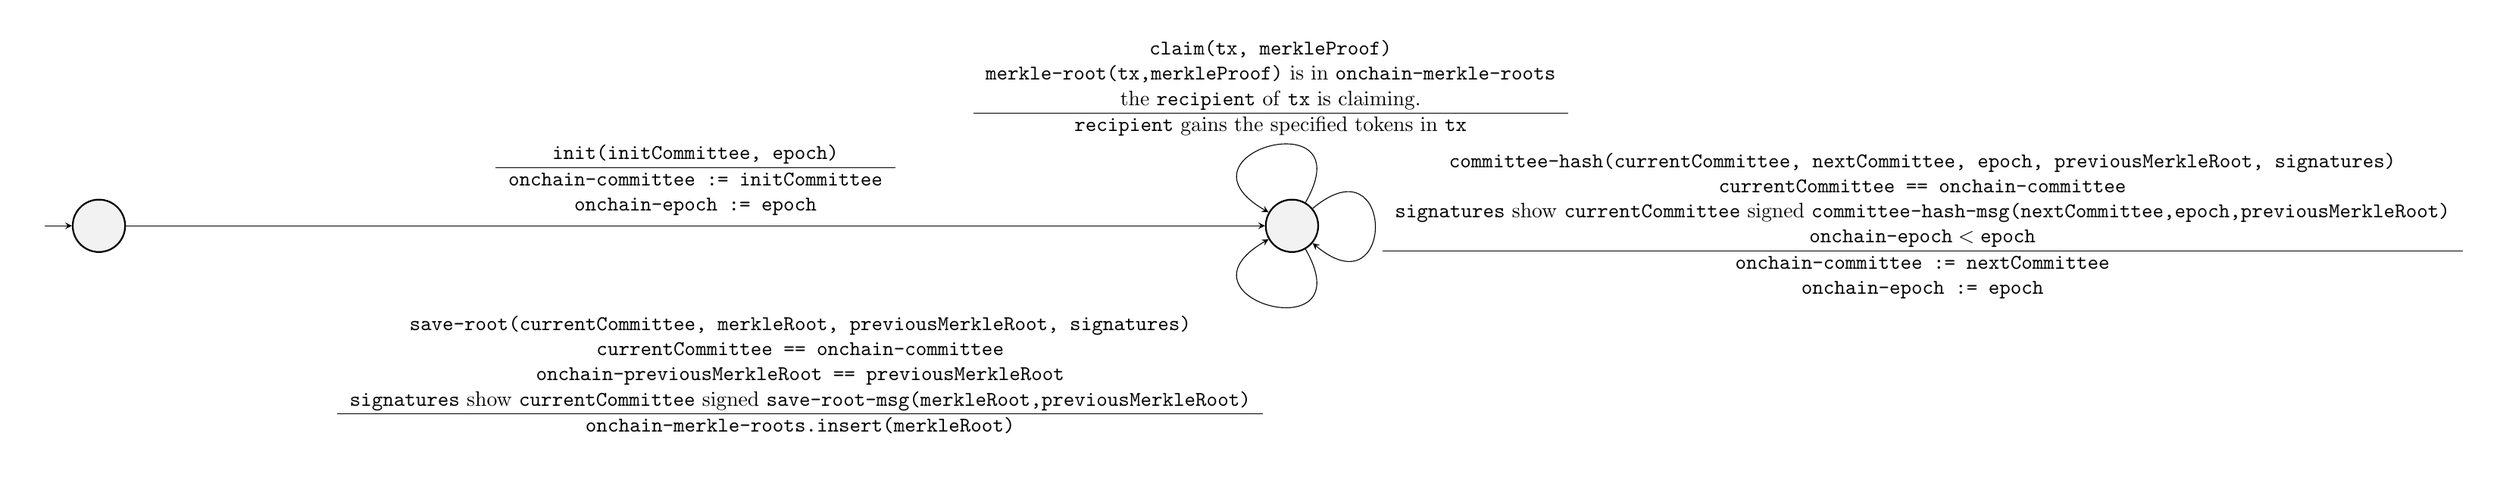
\begin{tikzpicture}[auto, background rectangle/.style={draw=white,fill=white}, show background rectangle]

        % Nodes
        \node[state, initial] (q1) {};
        \node[state, right of=q1] (q2) {};

        % edges
        \draw
            (q1)
                edge[above]
                node {
                    \begin{tabular}{c}
                        \texttt{init(initCommittee, epoch)}\\
                        \hline
                        \texttt{onchain-committee := initCommittee}\\
                        \texttt{onchain-epoch := epoch}
                    \end{tabular}
                    }
            (q2);
        \draw
            (q2)
                % edge[loop above]
                edge[out=60,in=150,looseness=8, above]
                node {
                    \begin{tabular}{c}
                        \texttt{claim(tx, merkleProof)}\\
                        \texttt{merkle-root(tx,merkleProof)} is in \texttt{onchain-merkle-roots} \\
                        the \texttt{recipient} of \texttt{tx} is claiming. \\
                        \hline
                        \texttt{recipient} gains the specified tokens in \texttt{tx}
                    \end{tabular}
                }
            (q2);
        \draw
            (q2)
                edge[out=300,in=210,looseness=8]
                node{
                    \begin{tabular}{c}
                        \texttt{save-root(currentCommittee, merkleRoot, previousMerkleRoot, signatures)}\\
                        \texttt{currentCommittee == onchain-committee}\\
                        \texttt{onchain-previousMerkleRoot == previousMerkleRoot}\\
                        \texttt{signatures} show \texttt{currentCommittee} signed \texttt{save-root-msg(merkleRoot,previousMerkleRoot)}\\
                        \hline
                        \texttt{onchain-merkle-roots.insert(merkleRoot)}
                    \end{tabular}
                }
            (q2);
        \draw
            (q2)
                % edge[loop right]
                edge[out=40,in=320, looseness=8]
                node{
                    \begin{tabular}{c}
                        \texttt{committee-hash(currentCommittee, nextCommittee, epoch, previousMerkleRoot, signatures)}\\
                        \texttt{currentCommittee == onchain-committee}\\
                        \texttt{signatures} show \texttt{currentCommittee} signed \texttt{committee-hash-msg(nextCommittee,epoch,previousMerkleRoot)}\\
                        $\texttt{onchain-epoch} < \texttt{epoch} $ \\
                        \hline
                        \texttt{onchain-committee := nextCommittee} \\
                        \texttt{onchain-epoch := epoch} \\
                    \end{tabular}
                }
            (q2);
    \end{tikzpicture}
\end{document}
